\mychapter{Estadística bidimensional}{Estadística bidimensional}{
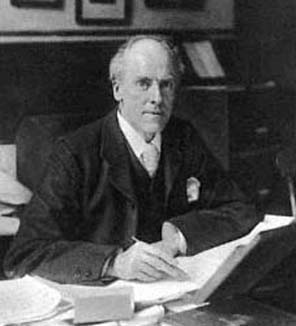
\includegraphics[width=4cm]{img-11/pearson}
\footnotesize

Karl Pearson (1857-1936)
}{chap:estadistica}

\section{Estadística descriptiva univariant}
\begin{theorybox}[Paràmetres estadístics]
	Donada una variable estadística $x_i$ amb cada valor repetit $f_i$ vegades (freqüència), es defineixen	
	
	\begin{minipage}{0.45\textwidth}
		\begin{itemize}
			\item \textbf{Nombre de dades:} $N=\sum_i f_i$
			\item \textbf{Mitjana aritmètica:} $\bar x=\dfrac{\sum_i f_i x_i}{N}$
			\item \textbf{Variància:} $Var=\dfrac{\sum_i f_i x^2_i}{N}-\bar x^2$
			\item \textbf{Desviació típica:} $\sigma=\sqrt{Var}$		
			\item \textbf{Coeficient de variació:} $CV = \dfrac{\sigma_x}{\bar x}$
		\end{itemize}
	\end{minipage}
	\hspace{0.3cm}
	\begin{minipage}{0.44\textwidth}
		\begin{itemize}
			\item \textbf{Moda:} El valor de $x$ més freqüent.
			\item \textbf{Mediana:} Valor de $x$ pel qual la {\normalfont \textit{freqüència acumulada}} assoleix el 50\%.
			\item \textbf{Rang:} La diferència entre els valors major i menor de $x$.
			
		\end{itemize}
	\end{minipage}
	
	La mitjana és el centre de gravetat de la distribució i la desviació típica ens dóna la \textbf{dispersió}. És a dir, ens diu com d'allunyades estan les dades respecte de la mitjana. 
	Podem pensar que una dada és ``normal'' si es troba dins l'interval de $x$ $(\bar x -\sigma, \bar x + \sigma)$.
\end{theorybox}


	\begin{mylist}
		\exer \mental Classifica les següents variables com a qualitatives o quantitatives, i aquestes últimes com a contínues o discretes. 
		\begin{tasks}
			\task Intenció de vot d'un partit. \hspace{0.25cm}\dotfill\hspace{1cm}
			%
			\task Nombre de correus electrònics que reps en un mes. \hspace{0.25cm}\dotfill\hspace{1cm}
			%
			\task Número de calçat. \hspace{0.25cm}\dotfill\hspace{1cm}
			%
			\task Nombre de quilòmetres recorreguts en cap de setmana. \hspace{0.25cm}\dotfill\hspace{1cm}
			%
			\task Marques de cervesa. \hspace{0.25cm}\dotfill\hspace{1cm}
			%
			\task Nombre d'empleats d'una empresa. \hspace{0.25cm}\dotfill\hspace{1cm}
			%
			\task Altura d'una persona. \hspace{0.25cm}\dotfill\hspace{1cm}
			%
			\task Temperatura d'un malalt. \hspace{0.25cm}\dotfill\hspace{1cm}
		\end{tasks}

	\answers{[Qualitativa, Quantitativa discreta, Quantitativa discreta, Quantitativa contínua, Qualitativa, Quantitativa discreta, Quantitativa contínua, Quantitativa contínua]}
	\end{mylist}


\begin{resolt}[E]{En un barri s'ha trobat que les famílies residents s'han distribuït, segons el número de membres, de la forma següent:\vspace{0.25cm}
		
	\begin{tabular}{|p{0.7in}|p{0.8in}|} \hline 
		\textbf{\textit{membres}} & \textbf{\textit{nº famílies}} \\ \hline 
		0-2 & 110 \\ \hline 
		2-4 & 200 \\ \hline 
		4-6 & 90 \\ \hline 
		6-8 & 75 \\ \hline 
		8-10 & 25 \\ \hline 
	\end{tabular}
	\vspace{0.25cm}
	
	\begin{itemize}
		\item[a)]  Representa un histograma.
		
		\item[b)]  Calcula la mitjana i la desviació típica.
	\end{itemize}
	}

	\begin{wrapfigure}{R}{0.3\textwidth} 
	\vspace{-0.75cm}
	\begin{center}
		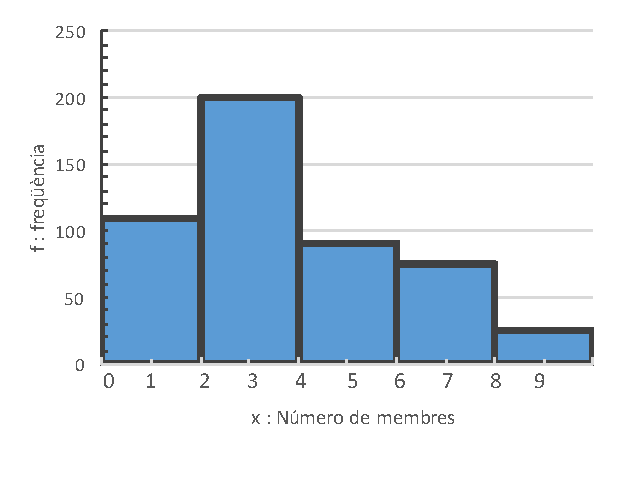
\includegraphics[width=0.26\textwidth]{img-11/histo1}
	\end{center}
\vspace{-0.5cm}
	\end{wrapfigure}

	Es tracta d'una variable discreta (número de membres) que s'ha agrupat en intervals. El número de famílies és la freqüència. Aleshores, el gràfic més adequat és fer un histograma.
	\vspace{0.24cm}
	
	Per calcular els paràmetres estadístics necessitam calcular \textbf{la marca de classe} que és el punt mitjà de cada interval.
	\begin{center}
		\begin{tabular}{|p{0.7in}|p{0.8in}|p{0.8in}|p{0.8in}|} \hline 
		$x_i$ & $f_i$ & $f_i x_i$ & $f_i x_i^2$\\ \hline 
		1 & 110 & 110 & 110 \\ \hline 
		3 & 200 & 600 & 1800 \\ \hline 
		5 & 90 & 450 & 2250\\ \hline 
		7 & 75 & 525 & 3675 \\ \hline 
		9 & 25 & 225 & 2025 \\ \hline\hline
		\rowcolor{lightgray} SUMES & 500 & 1910 & 9860\\ \hline 
	\end{tabular}
	\end{center}	\vspace{0.24cm}

	 La mitjana s'obté de $\bar x = \dfrac{1910}{500}=3.82$
	 
	 La desviació típica  $\sigma_x = \sqrt{ \dfrac{9860}{500}-3.82^2 }=2.26$
	 
	 El coeficient de variació és $CV = \dfrac{2.26}{3.82}=0.57$, aproximadament un 60\%.
	 
	\end{resolt}
	\vspace{1cm}

\begin{mylist}


\exer[1]  El govern desitja saber si el nombre de fills per família ha descendit respecte a la dècada anterior. Per a això s'ha demanant a 50 famílies pel nombre de fills i s'ha obtingut les dades següents. 
 
  \qquad	 2 \, 4 \, 2 \, 3 \, 1	 \qquad	  2 \, 4 \, 2 \, 3  \,0 \qquad	 2  \,2 \, 2 \, 3  \,2  \qquad	6 \, 2 \, 3 \, 2\,  2	\qquad  3 \, 2 \, 3  \,3 \, 4 	\par
  \qquad	 3 \, 3 \, 4  \,5 \, 2	 \qquad	  0  \,3   \,2  \,1 \, 2  \qquad	 3 \, 2\,  2 \, 3  \,1  \qquad	4  \,2  \,3 \, 2  \,4 	\qquad  3  \,3 \, 2 \, 2\,  1
 

\begin{tasks}
\task  Construeix la taula de freqüències amb aquestes dades. 
\task  Construeix el gràfic que consideris més adequat amb les freqüències.
\task  Calcula la mitjana i desviació típica del nombre de fills.
\end{tasks}
 
 
 \answers{\begin{tabular}{c|c|c|c|c|c|c|c}\hline
 $x$ & 0 & 1 & 2 & 3 & 4 & 5 & 6 \\\hline
 $f$ & 2 &4 & 21 & 15 & 6 & 1 &1 \\
\end{tabular}	

c) $\bar x =2.52$ i $\sigma=0.496$ fills.
 }
 
 
\exer[1] En un hospital es desitja fer un estudi sobre els pesos dels nounats. Per a això es recullen les dades de 40 nadons:

\pagebreak
 
 \begin{center}
 3.2  \, 3.7 \,  4.2 \,  4.6  \, 3.7 \qquad 3.0 \,  2.9 \,  3.1 \,  3.0  \, 4.5  \par 4.1  \, 3.8 \,  3.9\,   3.6 \,  3.2  \qquad 3.5 \,  3.0 \,  2.5\,   2.7\,    2.8 \par  3.0  \, 4.0 \,  4.5\,   3.5\,   3.5  \qquad 3.6  \, 2.9 \,  3.2 \,  4.2 \,  4.3 \par 4.1  \, 4.6\,   4.2 \,  4.5\,   4.3 \qquad 3.2 \,  3.7  \, 2.9 \,  3.1 \,  3.5 
\end{center}

\begin{tasks}
\task Construeix la taula de freqüències agrupant les dades en 5 intervals iguals.
\task Representa un histograma.
\task Calcula la mitjana i desviació típica. 
\end{tasks}

 \answers{\begin{tabular}{c|c|c|c|c|c}\hline
		$x$ & 2.5-3 & 3-3.5 & 3.5-4 & 4-4.5 & 4.5-5\\\hline
		$f$ & 6 & 10 & 11 & 8 & 5 \\
	\end{tabular}	
	
	c) $\bar x =3.7$ i $\sigma=0.62$ kg.
}

\end{mylist}

\section{Estadística bidimensional}
\begin{blueshaded}
	En nombroses ocasions ens interessa estudiar simultàniament dos o més caràcters de la població. En particular, volem saber quina
	  relació  existeix entre les variables. Aquest és l'objecte d'estudi de l'estadística bidimensional.
	
	Existeixen dos tipus de relació entre variables $\{x_i, y_i\}$:
	\begin{itemize}
		\item \textbf{Dependència funcional}: Existeix una llei funcional que relaciona les dues variables \linebreak $y_i  = f(x_i)$. \textit{A major pressió exercida, menor volum} $V=\frac{k}{P}$.
		\item \textbf{Correlació estadística}: No existeix cap llei exacta sinó que vindrà donada per una tendència. Per exemple, \textit{si els pares són alts, el normal és que els fills també ho siguin}.
	\end{itemize}

	Hi ha diversos tipus de correlació estadística:
	\begin{itemize}
		\item \textbf{Correlació positiva}: Quan $x_i$ augmenta, també ho fa $y_i$. Per exemple, \textit{les notes de l'examen de física i les notes de l'examen de matemàtiques.}
		\item \textbf{Correlació negativa}: Quan $x_i$ augmenta, $y_i$ disminueix. Per exemple, \textit{a major distància de la cistella de basquet, menor el nombre d'encerts.}
	\end{itemize}
	Cadascuna d'elles pot ésser correlació \textbf{forta} o correlació \textbf{feble}. Començarem l'estudi mesurant de forma qualitativa aquesta correlació. A mesura que avancem en el tema, però, aprendrem com descriure-la de forma quantitativa.
\end{blueshaded}
 
 \begin{mylist}
 		\exer \mental Per a cadascun dels casos següents analitza quin és el tipus de relació entre les variables (funcional o correlació). En cas de correlació indica si és positiva o negativa.
 	\begin{tasks}
 		\task El radi d'una esfera -- el costat d'aquesta
 		\task El nombre d'encerts d'un jugador de basquet -- La distància a la cistella.
 		\task Les notes de l'examen de matemàtiques -- Notes de l'examen de física.
 		\task La distància d'un trajecte en tren -- El preu el bitllet.
 		\task El pes dels alumnes de 1r de batxillerat -- La seva altura.
 		\task El nombre de membres de la família -- El preu del rebut d'aigua mensual.
 	\end{tasks}
 \end{mylist}
 
 \answers{[Funcional $D=2R$, Correlació negativa, Correlació positiva, Correlació positiva, Correlació positiva, Correlació positiva]}

\pagebreak
\subsection{Núvol de punts}
\begin{theorybox}
	Un núvol de punts s'obté de dibuixar els punts corresponents als parells $(x_i, y_i)$. 
	
	Aquest núvol ens ajuda a identificar el tipus de relació entre les variables:
	\begin{multicols}{7}
		\begin{center}
		\footnotesize
		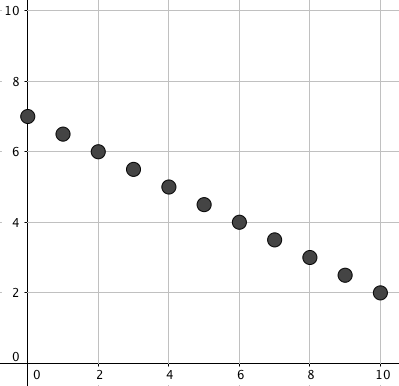
\includegraphics[width=2cm]{img-11/dep-fm}
		Funcional negativa
		
		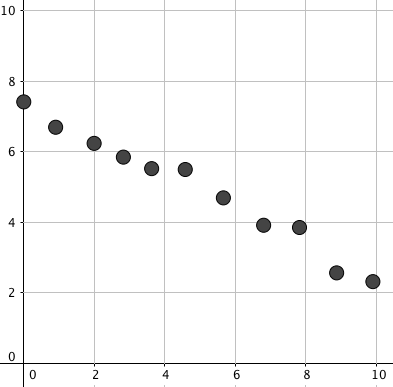
\includegraphics[width=2cm]{img-11/dep-cns}
		Correlació negativa forta
		
		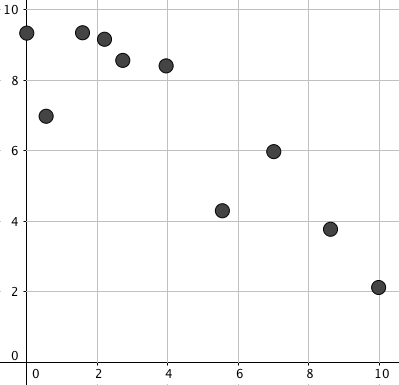
\includegraphics[width=2cm]{img-11/dep-cnfe}
		Correlació negativa feble
		
		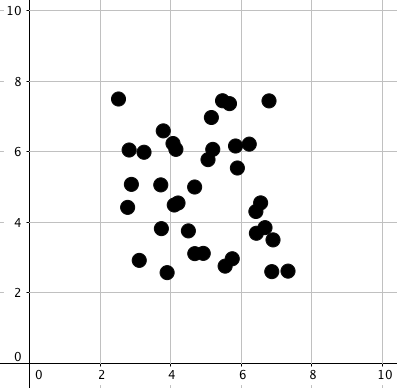
\includegraphics[width=2cm]{img-11/dep-no}
		Sense correlació
		
			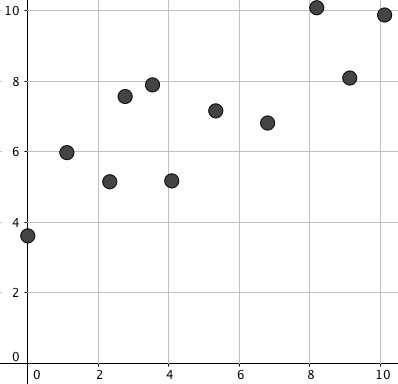
\includegraphics[width=2cm]{img-11/dep-cpw}
		Correlació positiva feble
		
			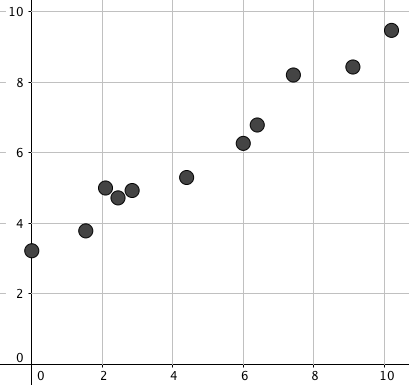
\includegraphics[width=2cm]{img-11/dep-cps}
		Correlació positiva forta
		
		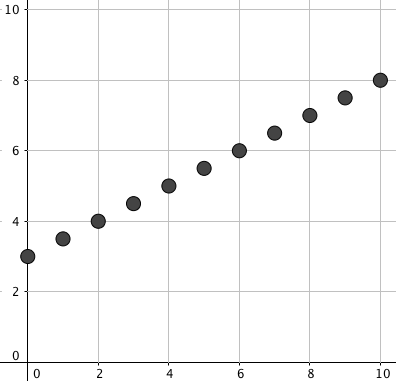
\includegraphics[width=2cm]{img-11/dep-fp}
		Funcional positiva
		\end{center}
	\end{multicols}
	Com més condensats estiguin els punts al voltant d'una línia recta diem que major és la correlació. Aquesta línia s'anomena \textbf{recta de regressió}. Si aquesta recta és creixent es diu que la correlació és positiva, mentres que si és decreixent la correlació és negativa.
	
	El \textbf{centre de gravetat} del núvol és a les mitjanes de les variables $G(\bar x, \bar y)$. Es compleix que la recta de regressió passa sempre pel centre de gravetat.
\end{theorybox}	

 
\begin{theorybox}[Núvol de bimbolles]
	Quan els punts $(x_i, y_i)$ venen agrupats en taula de doble entrada, en comptes de dibuixar un punt a  $(x_i, y_i)$, hi dibuixam una bimbolla amb radi proporcional a la freqüència del punt $f_i$.
	\begin{minipage}{0.6\textwidth}
		\begin{center}
			\begin{tabular}{|p{0.42in}|p{0.2in}|p{0.2in}|p{0.2in}|p{0.2in}|}
				\hline
				\rowcolor{lightgray} \diagbox{$x_i$}{$y_i$} & 1 & 2 & 3 & 4  \\ \hline
				\cellcolor{lightgray}	1 & 1 & 0 & 0 &  0 \\ \hline
				\cellcolor{lightgray}	2 & 0  &2  & 4 & 0  \\ \hline
				\cellcolor{lightgray}	3 & 0  &0  & 6 & 2  \\ \hline
				\cellcolor{lightgray}	4 & 0  &0  & 0 &  1 \\ \hline
			\end{tabular}
		\end{center}
	\end{minipage}
	\begin{minipage}{0.4\textwidth}
		\begin{center}
			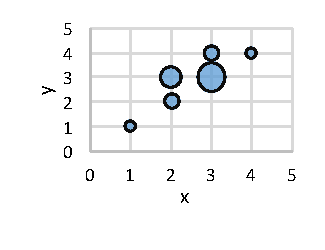
\includegraphics[width=0.8\textwidth]{img-11/nuvol-bimbolles}
		\end{center}
	\end{minipage}
\end{theorybox}

\begin{resolt}[E]{
En l'examen d'una assignatura que consta de part teòrica i part pràctica, les qualificacions van ser:
\vspace{0.25cm}

\begin{tabular}{|p{0.7in}|p{0.7in}|}
	 
\textbf{Teoria} & \textbf{Pràctica} \\ \hline
5 & 6\\ \hline
7 & 5 \\ \hline
6 & 8 \\ \hline
9 & 6\\ \hline
3 & 4\\ \hline
1 & 2\\ \hline
2 & 1\\ \hline
4 & 3\\ \hline
6 & 7\\ \hline 
\end{tabular}
\vspace{0.25cm}

 Dibuixa el núvol de punts i indica el tipus de relació.
}
 

Del núvol es dedueix que la dependència entre les variables és una correlació positiva d'intensitat moderada.

\begin{center}
	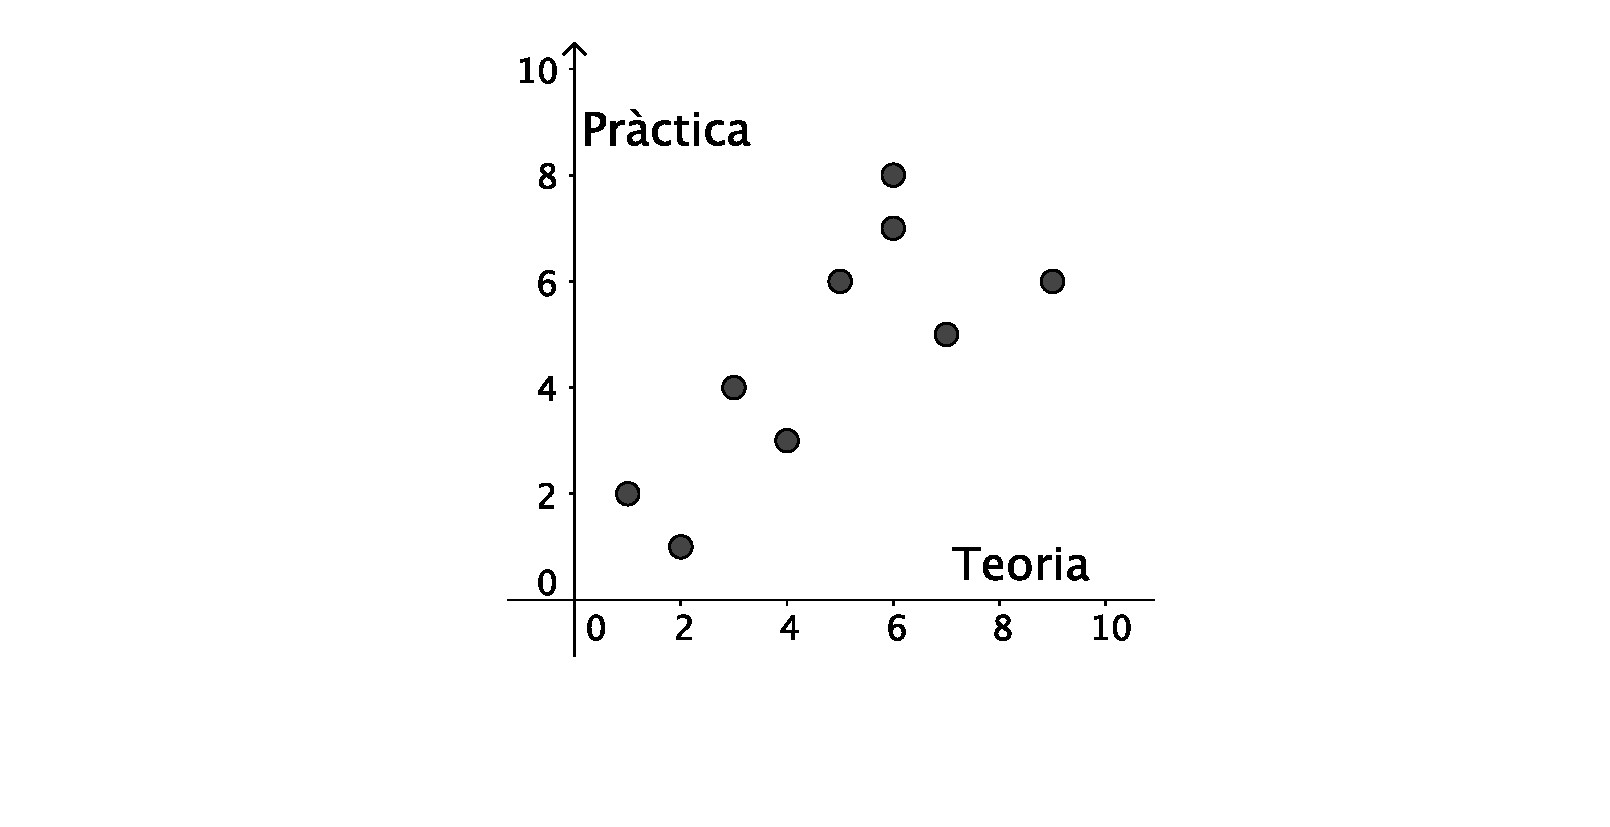
\includegraphics[width=0.3\textwidth]{img-11/nuvol-eg}
\end{center}

\end{resolt}
\vspace{0.5cm}

\begin{mylist}
	\exer En una zona residencial s'ha estudiat el nombre d'habitacions que té cada pis ($h$) i el nombre de persones que hi viuen ($p$). Aquests són els resultats
	\begin{center}
		\begin{tabular}{|p{0.3in}|| p{0.3in}|p{0.3in}|p{0.3in}|p{0.3in}|p{0.3in}|p{0.3in}|p{0.3in}|p{0.3in}|p{0.3in}|p{0.3in}|}
			\hline
			\cellcolor{lightgray} $h$ & 2 & 2 & 3 & 3 & 4 & 4 & 4 & 5 & 5 & 5\\ \hline
			\cellcolor{lightgray} $p$ & 1 & 2 & 2 & 3 & 3 & 4 & 5 & 4 & 5 & 6 \\ \hline
			\end{tabular}
	\end{center}
	Representa'ls mitjançant un núvol de punts i interpreta'l.
	
	\answers{Existeix una correlació positiva forta entre el nombre d'habitacions i les persones que hi viuen.\par 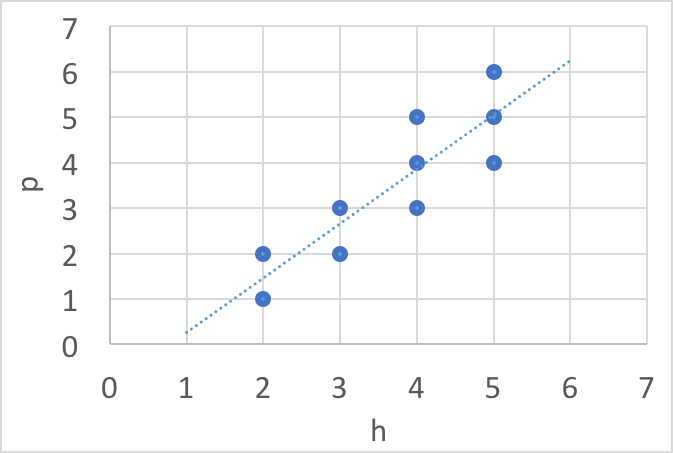
\includegraphics[width=0.4\textwidth]{img-sol/t11-5}}
	
	\exer En una mostra de 64 famílies s'ha estudiat el nombre de membres en edat laboral ($x$) i el nombre d'ells que es troben en actiu ($y$). Els resultats són a la taula. Representa un núvol.
	\begin{center}
	\begin{tabular}{|p{0.4in}|| p{0.7in}|p{0.7in}|p{0.7in}|p{0.7in}|}
		 \hline
		\rowcolor{lightgray} \diagbox{y}{x} & 1 & 2 & 3 & 4 \\ \hline \hline
		\cellcolor{lightgray} 1 & 6 & 10 & 12& 16\\ \hline
		 \cellcolor{lightgray} 2 & 0 & 2 & 5& 8\\ \hline
		 \cellcolor{lightgray} 3 & 0 & 0 & 1& 4\\ \hline
	\end{tabular}
	\end{center}

\answers{Existeix una correlació positiva feble entre les variables.\par 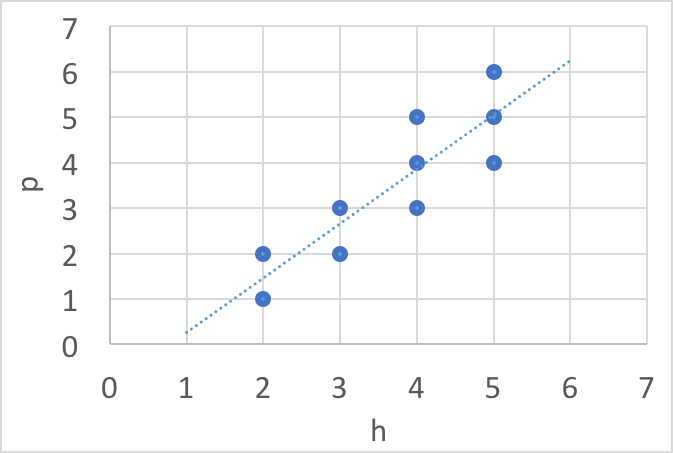
\includegraphics[width=0.4\textwidth]{img-sol/t11-5}}

\exer a) Traça a ull la recta de regressió per a cadascun dels casos següents

\begin{center}
	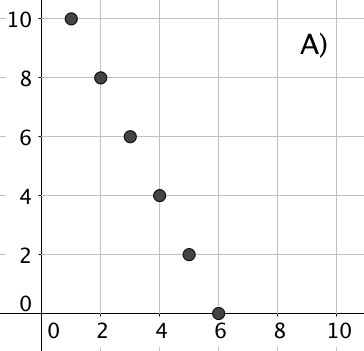
\includegraphics[width=0.3\textwidth]{img-11/dist-a}
	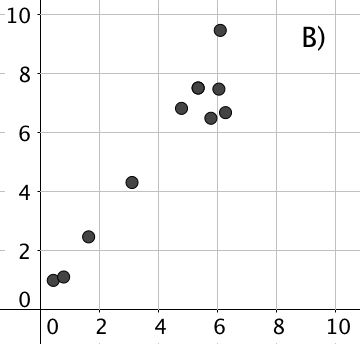
\includegraphics[width=0.3\textwidth]{img-11/dist-b}

	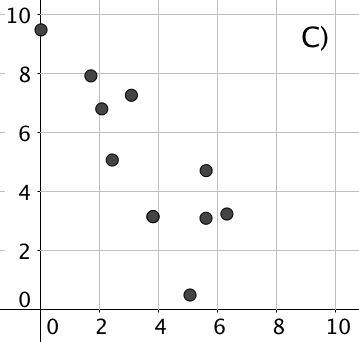
\includegraphics[width=0.3\textwidth]{img-11/dist-c}
	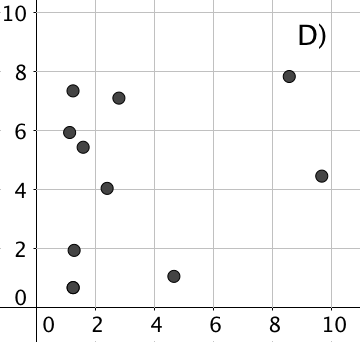
\includegraphics[width=0.3\textwidth]{img-11/dist-d}
\end{center}

b) Quin cas té correlació positiva i quin negativa?

c) Un cas és una relació funcional, quin? Troba la funció que relacionen les dues variables.

d) Ordena de menor a major les correlacions.

\answers{[Solució gràfica, Correlació \textbf{+}: B); D) aquesta darrera és quasi nul·la. Correlació \textbf{--}: A); C), A) és funcional $y=-2x+12$,
	Correlacions: $-1$=A) $<$ C) $<$ D) $<$ B) ]}
\end{mylist}



\pagebreak

\subsection{Covariància. Coeficient de regressió}
\begin{theorybox}
	A l'apartat anterior, el núvol de punts ens proporciona una forma de classificar la correlació entre les variables $\{x_i, y_i\}$ de forma qualitativa.
	
	Anomenam \textbf{covariància} al paràmetre estadístic que relaciona quantitativament la relació entre les variables:
	\begin{equation}
		\sigma_{xy} = \frac{\sum_i x_i \cdot y_i}{N} - \bar x \cdot \bar y
	\end{equation}
	on $N$ és el nombre de punts $(x_i, y_i)$  i $\bar x$, $\bar y$ les mitjanes de cada variable. 
	
	La covariància pot ésser negativa, zero o positiva segons els tipus de correlació que existeixi.
	
	Per poder quantificar millor l'intensitat de la correlació empram el \textbf{coeficient de correlació lineal o de Pearson} definit mitjançant
	\begin{equation}
		r = \frac{\sigma_{xy}}{\sigma_x \cdot \sigma_y} 
	\end{equation}
	Es compleix que $-1\leq r \leq 1$.
	\begin{center}
		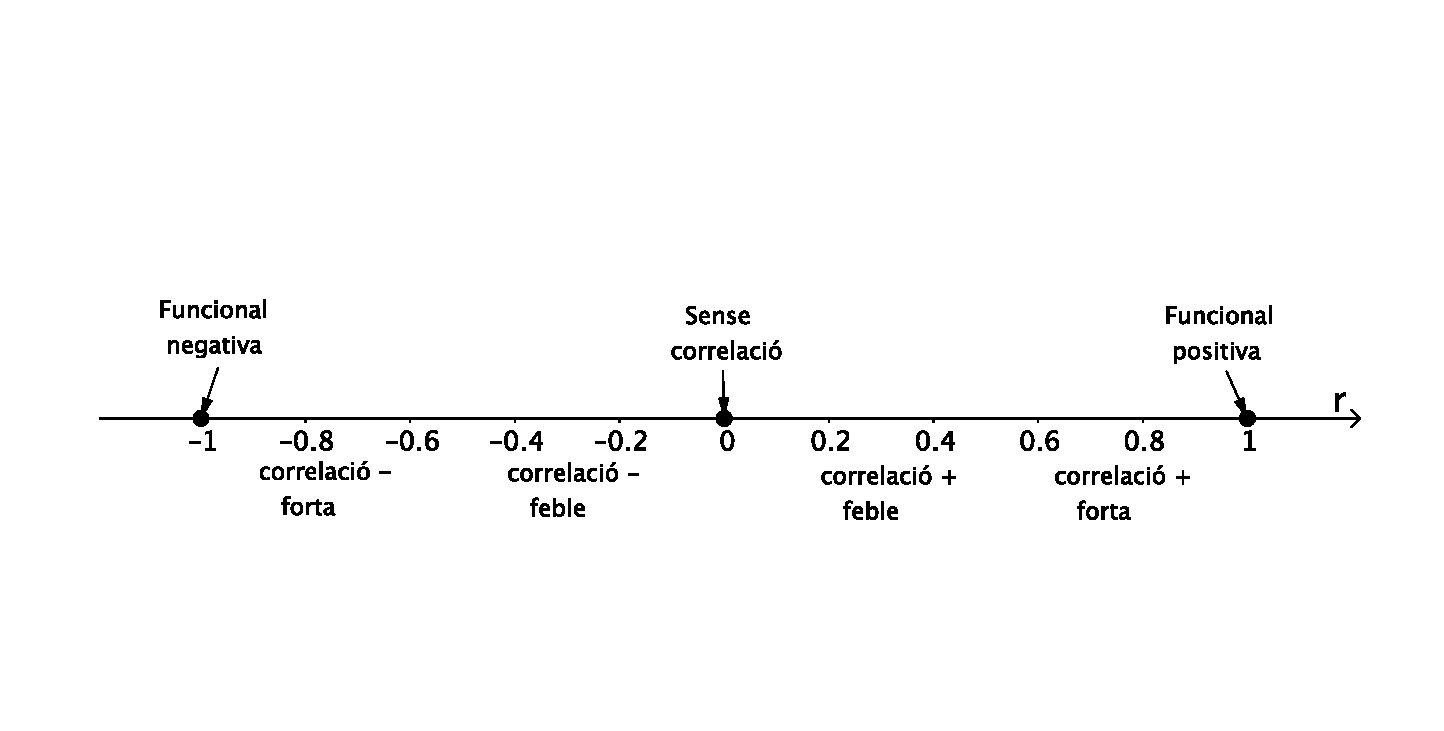
\includegraphics[width=0.8\textwidth]{img-11/coefcorr}
	\end{center}
\end{theorybox}	

\vspace{1cm}

\begin{resolt}{
	Calcula el coeficient de correlació entre les variables $x$: despeses en publicitat (milers d'euros) i $y$: vendes aconseguides (milers d'eurors)
	\vspace{0.25cm}
	
	\begin{tabular}{|p{0.7in}|p{0.7in}|}
	 \hline
	$x_i$ & $y_i$ \\ \hline
	1 & 10\\ \hline
	2 & 17 \\ \hline
	3 & 30\\ \hline
	4 & 28\\ \hline
	5 & 39\\ \hline
	6 & 47\\ \hline	 
\end{tabular}
}
Realitzam els càlculs de variància i covariància:\vspace{0.25cm}

\begin{tabular}{|p{0.7in}|p{0.7in}|p{0.7in}|p{0.7in}|p{0.7in}|} \hline
	
	$x_i$ & $y_i$ & $x_i^2$ & $y_i^2$ & $x_i y_i$ \\ \hline
	1 & 10 & 1 & 100  & 10 \\ \hline
	2 & 17 & 4 & 289 & 34 \\ \hline
	3 & 30 & 9 & 900 &  90 \\ \hline
	4 & 28 & 16 & 784 &  112\\ \hline
	5 & 39 & 25  & 1521 & 195 \\ \hline
	6 & 47 & 36  & 2209  &  282\\ \hline
	\rowcolor{lightgray} 21 & 171 & 91 & 5803 & 723 \\ \hline
\end{tabular}
\vspace{0.25cm}

Les mitjanes són: $\bar x = \dfrac{21}{6}=3.5$, $\bar y = \dfrac{171}{6}=28.5$.\vspace{0.25cm}

Les desviacions típiques són:
\begin{center}
	$\sigma_x = \sqrt{ \dfrac{91}{6} - 3.5^2}=1.71$, 
	$\sigma_y = \sqrt{ \dfrac{5803}{6} - 28.5^2}=12.45$\vspace{0.25cm}
\end{center}

La covariància és   $\sigma_{xy} = \dfrac{723}{6} - 3.5 \cdot 28.5 = 20.75$ \vspace{0.25cm}

El coeficient de correlació $r = \dfrac{20.75}{1.71 \cdot 12.45}=0.97$. És una correlació molt forta positiva ja que és proper a 1. \vspace{0.25cm}

\end{resolt}
\vspace{0.5cm}


\begin{mylist}
	\exer  L'evolució de l'IPC (índex de preus al consum) i la taxa d'inflació en els mesos indicats d'un determinat any, va ser:
 
 \begin{tabular}{|p{1.0in}|p{0.6in}|p{0.6in}|p{0.6in}|p{0.6in}|p{0.6in}|p{0.6in}|} \hline 
		\textbf{} & Gener & Febrer & Març & Abril & Maig & Juny \\ \hline 
		\textbf{IPC} & 0.7 & 1.1 & 1.7 & 2 & 1.9 & 1.9 \\ \hline 
		\textbf{Taxa inflació} & 6 & 6 & 6.3 & 6.2 & 5.8 & 4.9 \\ \hline 
	\end{tabular}
	
	\begin{tasks}
		\task  Representa el núvol de punts.
		%
		\task  Calcula el coeficient de correlació entre l'IPC i la taxa d'inflació.
		%
		\task  Es pot estimar la taxa de inflació a partir de l'IPC?
	\end{tasks}

\answers[cols=1]{[\mbox{} \par \ggblink{https://goo.gl/hpSTWs}, $r=-0,24$, Pràcticament no existeix cap correlació entre les variables i per tant no té sentit estimar la taxa a partir de l'IPC.]}
\end{mylist}


\subsection{Rectes de regressió}
\begin{theorybox}
	Com hem dit, la recta de regressió passa pel \textbf{centre de gravetat} del núvol de punts $(\bar x, \bar y)$ i és la recta que "millor ajusta". L'equació punt-pendent d'aquesta recta serà de la forma $y-\bar y = m (x-\bar x)$ on $m$ és el pendent de la recta. El criteri que s'utilitza per determinar el pendent que millor ajusta s'anomena el \textbf{mètode dels mínims quadrats}. Aquest mètode es basa en imposar que la suma de les distàncies al quadrat de cadascun dels punts a la recta sigui mínima. El resultat que s'obté és:
	\begin{equation}
		y=\bar y + \frac{\sigma_{xy}}{\sigma_x^2}(x-\bar x)
	\end{equation}
	S'anomena la recta de regressió de Y sobre X.
	
	La recta de regressió s'utilitza per fer prediccions d'una variable coneguda l'altra. La predicció serà més bona o fiable  com més s'apropi a $\pm 1$ el coeficient de correlació $r$.
\end{theorybox}	

\begin{mylist}
	
	\vspace{-1.5cm}
	\exer[1] \begin{minipage}[t]{0.7\textwidth}
		La \textit{Llei de Hooke} relaciona l'allargament d'una molla amb la força que hi aplicam $F=k x$ on $k$ és la constant d'elàstica. Hem anant penjat a la molla pesos de diferent valors i hem anotat l'allargament
		
		\begin{tabular}{|p{1.5in}|p{0.4in}|p{0.4in}|p{0.4in}|p{0.4in}|p{0.4in}|} \hline 
			\textbf{Allargament $x$ (m)} & 0 & 0.06 & 0.2 & 0.3 & 0.6  \\ \hline 
			\textbf{Pes $F$ (N)} & 0 & 0.45 & 1.1 & 1.47 & 2.95  \\ \hline 
		\end{tabular}
		\vspace{0.25cm}
		\begin{tasks}
			\task Calcula la recta de regressió i estima el valor de la constant elàstica de la molla.
			\task  Estima l'allargament que produiria un pes de 2 N. 
		\end{tasks}
		
	\end{minipage}
	\begin{minipage}{0.16\textwidth}
		\centering
		\vspace{2.25cm}
		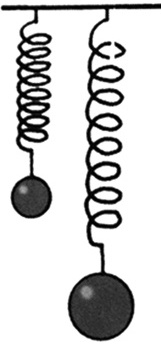
\includegraphics[width=0.4\textwidth]{img-11/hooke}
	\end{minipage}

 \answers{$y=1.194+4.78(x-0.232)$, el pendent és la constant elàstica $k=4.78$ N/m. L'allargament per a $y=2$ N és $x=40$ cm. És bastant fiable ja que $r=0,998$.}
 \vspace{0.5cm}
	
	\exer  La taula següent mostra el nombre de gèrmens patògens per centímetre cúbic d'un determinat cultiu segons el temps transcorregut.
	
	\begin{tabular}{|p{1.5in}|p{0.5in}|p{0.5in}|p{0.5in}|p{0.5in}|p{0.5in}|p{0.5in}|} \hline 
		\textbf{Nombre d'hores} & 0 & 1 & 2 & 3 & 4 & 5 \\ \hline 
		\textbf{Nombre de gèrmens} & 20 & 26 & 33 & 41 & 47 & 53 \\ \hline 
	\end{tabular}
	
	\begin{tasks}
		\task  Calcula la recta de regressió del nombre de gèrmens en funció del temps.
		%
		\task  Quina quantitat de gèrmens per centímetre cúbic és previsible trobar quan transcorrin 6 hores? És bona aquesta predicció?
	\end{tasks}

\answers[cols=1]{[$y=6,743x+19,81$ \par \ggblink{https://goo.gl/ExXjiX},
	quan $x=6$ estimam que $y=60,3$ gèrmens/cm$^3$. La predicció és molt bona perquè tenim una correlació forta amb $r=0,99894$.]}

\pagebreak
	
	\exer[1]  En un dipòsit cilíndric, l'altura de l'aigua que conté varia a mesura que passa el temps segons les dades recollides en la taula:
	\answers{a) $r=-0.997$ correlació negativa forta; \quad b) Recta de regressió $y=-0.2632 x+10.37$, altura $y=8.84$ m.  \quad c) $x=66$ hores}
	
	
	\begin{tabular}{|p{1.1in}|p{0.7in}|p{0.7in}|p{0.7in}|p{0.7in}|p{0.7in}|} \hline 
		\textbf{Temps: \textit{h}} & 8 & 22 & 27 & 33 & 50 \\ \hline 
		\textbf{Altura: \textit{m}} & 17 & 14 & 12 & 11 & 6 \\ \hline 
	\end{tabular}
	
	\begin{tasks}
		\task  Troba el coeficient correlació entre el temps i l'altura. Interpreta'l.
		%
		\task  Quina altura s'aconsegueix transcorregudes 40 hores?
		%
		\task  Quan l'altura assoleix 2 m, sona una alarma. Quant de temps ha de transcórrer perquè soni l'alarma?
	\end{tasks}

\answers[cols=1]{[$r=-0,9965$ és una correlació negativa forta \par \ggblink{https://goo.gl/i694tR}, 
	Primer calculam la recta de regressió lineal $y=-0,2632 x + 19,37$ i feim la predicció $y(40)=8,84$ metres, També utilitzam la recta de regressió però ara aïllam $x=66$ hores.]}
	
	
	\exer La taula següent relaciona el nombre atòmic de diversos metalls amb la seva densitat
 
\begin{tabular}{|p{1.1in}|p{0.3in}|p{0.3in}|p{0.3in}|p{0.3in}|p{0.3in}|p{0.3in}|p{0.3in}|p{0.3in}|} \hline 
	\textbf{Element}  & K & Ca & Ti & V & Mn & Fe & Co & Ni  \\ \hline 
	\textbf{N. atòmic} & 19 &20  & 22 & 23 & 25& 26 &27 & 28\\ \hline 
	\textbf{Densitat} & 0.86 & 1.54 & 4.50 & 5.60 & 7.11 & 7.88 & 8.70 & 8.80 \\ \hline 
	
\end{tabular}

\begin{tasks}
	\task  Representa els punts i troba el coeficient de regressió.
	%
	\task  Mitjançant la recta de regressió, estima la densitat del crom amb nombre atòmic 24.
\end{tasks}	
	
\answers[cols=1]{[El coeficient de regressió $r=0,9857$ és una correlació positiva forta\par \ggblink{https://goo.gl/5nRcAv},
	La recta de regressió lineal $y=0,9319 x-16,509$ estimam el valor de $y$ quan $x=24$ i trobam $y=5,857$. Segons la wikipèdia té una densitat de 7,140 g/cm$^3$.\par \ggblink{https://es.wikipedia.org/wiki/Cromo}]}

\end{mylist}





\begin{resolt}[E]{
En l'examen d'una assignatura que consta de part teòrica i part pràctica, les qualificacions de nou alumnes van ser:
\vspace{0.25cm}

\begin{tabular}{|p{0.7in}|p{0.7in}|}
	 \hline
	\textbf{Teoria} & \textbf{Pràctica} \\ \hline
	5 & 6\\ \hline
	7 & 5 \\ \hline
	6 & 8 \\ \hline
	9 & 6\\ \hline
	3 & 4\\ \hline
	1 & 2\\ \hline
	2 & 1\\ \hline
	4 & 3\\ \hline
	6 & 7\\ \hline 
\end{tabular}
\vspace{0.25cm}

Calcula la recta de regressió Pràctica en funció de Teoria.
Utilitza-la per predir la nota de pràctica d'un alumne que obtingués 4.75 en teoria. Quan de fiable és la predicció?	

}

Realitzam els càlculs de variància i covariància:\vspace{0.25cm}

\begin{tabular}{|p{0.7in}|p{0.7in}|p{0.7in}|p{0.7in}|p{0.7in}|} \hline
	
	$x_i$ & $y_i$ & $x_i^2$ & $y_i^2$ & $x_i y_i$ \\ \hline
	5 & 6 & 25 & 36 & 30 \\ \hline
	7 & 5 & 49 & 25 & 35 \\ \hline
	6 & 8 & 36 & 64 & 48 \\ \hline
	9 & 6 & 81 & 36 & 54 \\ \hline
	3 & 4 & 9  & 16 & 12 \\ \hline
	1 & 2 & 1  & 4  & 2 \\ \hline
	2 & 1 & 4  & 1  & 2 \\ \hline
	4 & 3 & 16 & 9  &12\\ \hline
	6 & 7 & 36 & 49 & 42\\ \hline\hline
	\rowcolor{lightgray} 43 & 42	& 257 & 240 & 237 \\ \hline
\end{tabular}
\vspace{0.25cm}

Les mitjanes són: $\bar x = \dfrac{43}{9}=4.78$, $\bar y = \dfrac{42}{9}=4.67$.\vspace{0.25cm}

Les desviacions típiques són:
\begin{center}
 $\sigma_x = \sqrt{ \dfrac{257}{9} - 4.78^2}=2.39$, $\sigma_y = \sqrt{ \dfrac{240}{9} - 4.67^2}=2.21$\vspace{0.25cm}
\end{center}

La covariància és   $\sigma_{xy} = \dfrac{237}{9} -4.78 \cdot 4.67 = 4.04$ \vspace{0.25cm}

El coeficient de correlació $r = \dfrac{4.04}{2.39 \cdot 2.21}=0.763$\vspace{0.25cm}

La recta de regressió $y = 4.67 + 0.705\cdot(x-4.78)$.\vspace{0.25cm}

La predicció sabent que $x=4.75$ és  $y = 4.67 + 0.705\cdot(4.75-4.78)=4.65$. És poc fiable donat que el coeficient de correlació és menor que $0.9$. 
\end{resolt}

\pagebreak
\mbox{}

\vspace*{-2.65cm}


\begin{mylist}
	
 \exer \begin{minipage}[t]{0.7\textwidth}
 	Per \textit{trobar la gravetat de la Terra} podem utilitzar un pèndol format per una massa penjada a l'extrem d'un fil prim de longitud $l$. Mesuram el període d'oscil·lació en funció de la longitud de la corda
 	
 	\begin{tabular}{|p{1.in}|p{0.5in}|p{0.5in}|p{0.5in}|p{0.5in}|p{0.5in}|} \hline 
 		\textbf{Longitud $x$ (m)} 		   & 0.10  & 0.20 & 0.30 & 0.3 & 0.4  \\ \hline 
 		\textbf{Període$^2$ $T^2$ (s$^2$)} & 0.386 & 0.80 & 1.1 & 1.19 & 1.60  \\ \hline 
 	\end{tabular}
 	\vspace{0.25cm}
 	\begin{tasks}
 		\task  Calcula la recta de regressió i estima el valor de la acceleració de la gravetat $g$ sabent que  $T^2 = \frac{4\pi^2}{g} l$. 
 		\task  Estima el període d'un pèndol de longitud 0.75 m. 
 	\end{tasks}
 \end{minipage}
 \begin{minipage}{0.3\textwidth}
 	\centering
 	\vspace{2.5cm}
 	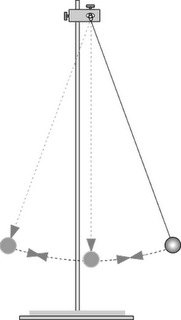
\includegraphics[width=0.5\textwidth]{img-11/pendol}
 \end{minipage}
  
	
	\answers{[La recta de regressió és $y=3,9585x-0,014$. Tenim una correlació positiva forta. \par \ggblink{https://goo.gl/cY7x1L},
		Segons la teoria el pendent de la recta de regressió ha d'esser igual a $3,9585=\dfrac{4\pi^2}{g}$; d'aquí podem aïllar $g=9,973$ m/s$^2$ que s'assembla bastant al $9,8$ del llibres de text.\par
		Amb la recta de regressió estimam la $y$ quan $x=0.75$ m; $y=2,9548$ s$^2$; el període és l'arrel quadrada d'aquest nombre $T=1,719$ s. 
		]}
	
\end{mylist}
 
\begin{activitats}
	\begin{mylist}
		 
\exer  En llançar 200 vegades un dau es va obtenir la següent distribució de freqüències. 
 
\begin{tabular}{|p{0.2in}|p{0.2in}|p{0.2in}|p{0.2in}|p{0.2in}|p{0.2in}|p{0.2in}|} \hline
	
	$x_i$ &  1 & 2 & 3 & 4 & 5  & 6 \\ \hline
    $f_i$ & \textit{a} & 32 & 35  & 33 & \textit{b}  & 35\\ \hline
 
\end{tabular} 

\noindent Troba la mediana i la moda de la distribució, sabent que la mitjana aritmètica és 3.6.

\answers{$N=\sum_i f_i=200$; llavors $a+b+135=200$. Després la mitjana\par $\dfrac{a+2\cdot 32 + 3 \cdot 35 + 4\cdot 33 + 5b+ 6\cdot 35}{200}=3.6$  $\rightarrow$  $511+a+5b=720$.\par Resolem el sistema d'equacions i trobam $a=29$ i $b=36$.\par
La moda és $Mo=5$; la mediana és $Me=4$}

\exer  Les següents dades són mesures de la capacitat cranial d'un grup d'homínids: 

84, 49,61, 40, 83, 67, 45, 66, 70, 69, 80, 58, 68, 60, 67, 72, 73, 70, 57, 63, 70, 78, 52, 67, 53, 67, 75, 61, 70, 81, 76, 79, 75, 76, 58, 31.
\begin{tasks}
\task   Agrupa les dades en 6 intervals iguals de 30 fins 90.
	%
\task  Calcula la mitjana. 
 %
\task  Calcula la variància i la desviació estàndard de la mostra.
\end{tasks}
\answers{ \begin{tabular}{|c|c|}\hline
		\rowcolor{lightgray} $x$ & $y$ \\\hline
		$[30,\;40 )$ & 1\\ \hline 
		$[40,\;50 )$ & 3\\ \hline 
		$[50,\;60 )$ & 5\\ \hline 
		$[60,\;70 )$ & 11\\ \hline 
		$[70,\;80 )$ & 12\\ \hline 
		$[80,\;90 )$ & 4\\ \hline 
	\end{tabular}
	\par
	$N= 36 $; $\sum f\cdot x= 2400 $; $\sum f\cdot x^2= 165300 $
	\par
	$\bar x= 66.67 $;  Var$= 147.22 $; $\sigma= 12.13 $; C.V.= 0.18}

\exer Les següents dades procedeixen d'un estudi de contaminació de l'aire. 

\noindent 6.5 \quad 2.1 \quad 4.4 \quad 4.7 \quad 5.3 \quad 2.6 \quad 4.7 \quad 3.0 \quad 4.9 \quad 8.6 \quad 5.0 \quad 4.9 \quad 4.0 \quad 3.4 \quad 5.6 \quad 4.7 \quad 2.7 \quad 2.4 \quad 2.7 \quad 2.2 \quad 5.2 \quad 5.3 \quad 4.7 \quad 6.8 \quad 4.1 \quad 5.3 \quad 7.6 \quad 2.4 \quad 2.1 \quad 4.6 \quad 4.3 \quad 3.0 \quad 4.1 \quad 6.1 \quad 4.2
 

\begin{tasks}
	\task Agrupa les dades en 4 intervals iguals de 2 fins 10.
	\task Construeix un histograma.
	\task Calcula la mitjana i la desviació típica. 
\end{tasks} 
\answers{\begin{tabular}{|c|c|}\hline
		\rowcolor{lightgray} $x$ & $y$ \\\hline
		$[2,\;4 )$ & 11\\ \hline 
		$[4,\;6 )$ & 19\\ \hline 
		$[6,\;8 )$ & 4\\ \hline 
		$[8,\;10 )$ & 1\\ \hline 
	\end{tabular}
	\par
	$N= 35 $; $\sum f\cdot x= 165 $; $\sum f\cdot x^2= 851 $
	\par
	$\bar x= 4.71 $;  Var$= 2.09 $; $\sigma= 1.45 $; C.V.= 0.31 \par \ggblink{https://goo.gl/Q6BEy9} }
 
\exer Les dades següents són les qualificacions obtingudes pels 24 estudiants d'un grup de 1r de batxillerat en les assignatures de Matemàtiques i Llengua.
 
\hspace{-0.5cm}\begin{tabular}{|p{0.3in}|p{0.12in}|p{0.12in}|p{0.12in}|p{0.12in}|p{0.12in}|p{0.12in}|p{0.12in}|p{0.12in}| } \hline 
\textbf{Mat} &  4 & 5 & 5 & 6 & 7 & 7 & 7 & 7  \\ \hline 
\textbf{Llen} & 3 & 5 & 6 & 7 & 7 & 7 & 7 & 8  \\ \hline\hline  
\textbf{Mat} & 8 & 8 & 8 & 8 & 9 & 9 & 9 & 9  \\ \hline 
\textbf{Llen} & 8 & 8 & 8 & 8 & 8 & 8 & 8 & 10  \\ \hline \hline 
\textbf{Mat} &  7 & 7 & 8 & 8 & 10 & 10 & 9 & 9 \\ \hline 
\textbf{Llen} & 8 & 8 & 7 & 7 & 9 & 10 & 9 & 8 \\ \hline 
\end{tabular}

\begin{tasks}
\task  Proporció d'estudiants  que obté més d'un cinc en ambdues assignatures, proporció d'estudiants  que obté més d'un cinc en Matemàtiques, proporció estudiants que obté més d'un cinc en Llengua.
\task  Són independents les qualificacions de  Matemàtiques i Llengua?
\task  Representa gràficament.
\task  Calcula el coeficient correlació.
\end{tasks}

\answers{[El 88 \% obté més de 5 en ambdues assignatures; El 88 \% en matemàtiques i el 92 \% en llengua,
	Estan fortament relacionades, Gràfic, Coeficient de correlació = 0,87 positiu i molt alt.
 }


\exer  El volum d'estalvi i la renda del sector famílies en milions d'euros  per al període 2005-2012 van ser:
 

\hspace{-1cm}{\scriptsize\begin{tabular}{|p{0.3in}|p{0.15in}|p{0.15in}|p{0.15in}|p{0.15in}|p{0.15in}|p{0.15in}|p{0.15in}|p{0.15in}| } \hline 
\textbf{Anys} & 05 & 06 & 07 & 08 & 09 & 10 & 11 & 12  \\ \hline 
\textbf{Estalvi} & 1'9 & 1'8 & 2'0 & 2'1 & 1'9 & 2'0 & 2'2 & 2'3   \\ \hline 
\textbf{Renta} & 20'5 & 20'8 & 21'2 & 21'7 & 22'1 & 22'3 & 22'2 & 22'6   \\ \hline 
\end{tabular}}

\begin{tasks}
\task  Recta regressió de l'estalvi sobre la renta.
%
\task  Recta de regressió de la renta sobre l'estalvi.
%
\task  Per a l'any 2015 se suposa que la renta era de 24.1 milions d'euros. Quin serà l'estalvi esperat per a l'any 2015?
%
\task  Estudiar la fiabilitat de la predicció anterior.
\end{tasks}

\answers{[$y=3,2564 x + 15,0807$,
	$x=0,155828 - 1,35257$,
	Si utilitzam la recta Y sobre X: $x=2,77$ \par
	Si utilitzam la recta Y sobre X: $x=2,40$,
	La predicció és acceptable tenint present que $r=0,7123$. A major valor de $r$ menor la diferència entre les dues prediccions anteriors.  \par 
	\ggblink{https://goo.gl/c1dcec}]}


\exer  Es va mesurar el temps en segons que van trigar a gravar-se els mateixos 18 fitxers en un llapis USB \textit{X} i en un disc dur exterior \textit{Y}.

\hspace{-1cm}\begin{tabular}{|p{0.15in}|p{0.15in}|p{0.15in}|p{0.15in}|p{0.15in}|p{0.15in}|p{0.15in}|p{0.15in}|p{0.15in}|p{0.15in}|} \hline 
\textbf{\textit{X}} & 1'2 & 1 & 1'1 & 0'5 & 1'1 & 1'5 & 1 & 1'4 & 1'4  \\ \hline 
\textbf{\textit{Y}} & 1'3 & 1'1 & 1'2 & 0'4 & 1'2 & 1'4 & 1'1 & 1'6 & 1'6   \\ \hline 
\end{tabular}



\hspace{-1cm}\begin{tabular}{|p{0.15in}|p{0.15in}|p{0.15in}|p{0.15in}|p{0.15in}|p{0.15in}|p{0.15in}|p{0.15in}|p{0.15in}|p{0.15in}|} \hline 
\textbf{\textit{X}} & 0'3 & 1'5 & 1'4 & 1'1 & 1'2 & 1'2 & 0'4 & 0'5 & 1'3   \\ \hline 
\textbf{\textit{Y}} & 0'3 & 1'6 & 1'3 & 1'1 & 1'3 & 1'1 & 0'4 & 0'4 & 1'4  \\ \hline 
\end{tabular}

\begin{tasks}	
\task  Representa gràficament les dades i comenta el resultat obtingut.
\task  Si un fitxer triga 0'8 segons a gravar-se en el primer tipus de memòria, quants segons trigaria a gravar-se en el segon tipus? Donar una mesura de fiabilitat. 
\end{tasks}

\answers[cols=1]{[Hi ha una correlació positiva forta\par 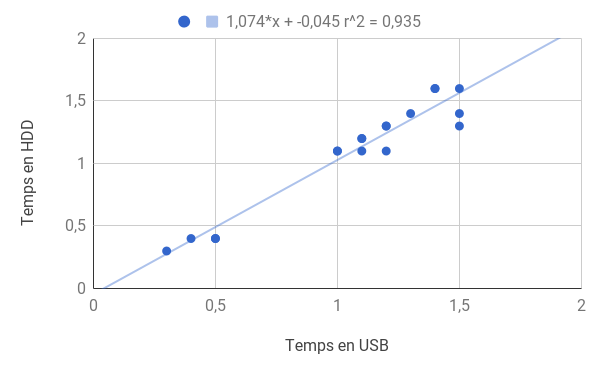
\includegraphics[width=0.4\textwidth]{img-sol/t11-19}\par
	\ggblink{https://goo.gl/3AMzyc}
	,
	La recta de regressió és $y=1,0736 x -0,04522$. L'estimació $y(x=0,8)=0,8137$.\par
	L'estimació és bastant fiable ja que el coeficient de correlació és alt $r=0,967$.
	]}

\exer S'han estudiat els errors comesos per un grup de 117 persones en dues proves: d'ortografia $x$ i de càlcul numèric $y$. Els resultats són els de 
la taula de doble entrada següent

\begin{center}
\begin{tabular}{c|c|c|c|c|c}
\rowcolor{lightgray} \diagbox{$y_i$}{$x_i$} & 0 & 1 & 2 & 3 & 4 \\ \hline
\cellcolor{lightgray}    	 0 & 24 & 6  &1 & 0 & 0 \\ \hline
\cellcolor{lightgray}	    1 & 11 & 19 &2 & 3 & 0 \\ \hline
\cellcolor{lightgray} 		2 & 7 & 8   &6 & 2 & 0 \\ \hline
\cellcolor{lightgray} 		3 & 2 & 3  &3 & 7& 1 \\ \hline
\cellcolor{lightgray} 		4 & 1 & 0  &2 & 4& 5 \\ \hline
\end{tabular}
\end{center}

\begin{tasks}
	\task Troba les distribucions marginals de $x$ i $y$
	\task Troba la distribució de $x$ condicionada a $y<2$.
	\task Calcula el coeficient de correlació lineal
\end{tasks}

\answers{[\begin{tabular}{|c|c|}\hline
		\rowcolor{lightgray} $x$ & $f$ \\\hline
		$0$ & 45\\ \hline
		$1$ & 36\\ \hline 
		$2$ & 14\\ \hline 
		$3$ & 16\\ \hline 
		$4$ & 6\\ \hline 
	\end{tabular}
	\hspace{0.25cm}
	\begin{tabular}{|c|c|}\hline
		\rowcolor{lightgray} $y$ & $f$ \\\hline
		$0$ & 31\\ \hline
		$1$ & 35\\ \hline 
		$2$ & 23\\ \hline 
		$3$ & 16\\ \hline 
		$4$ & 12\\ \hline 
	\end{tabular},
	%%
	\begin{tabular}{|c|c|}\hline
		\rowcolor{lightgray} $x | y<2$ & $f$ \\\hline
		$0$ & 35\\ \hline
		$1$ & 25\\ \hline 
		$2$ & 3\\ \hline 
		$3$ & 3\\ \hline 
		$4$ & 0\\ \hline 
	\end{tabular},
	%%
	$r=0.6743$ és una correlació positiva moderada \par \ggblink{https://goo.gl/qdmVsS}
	]}

\exer En una mostra de 64 famílies, s'han estudiat el nombre de membres en edat laboral, $x$, i el nombre d'ells que estan
en actiu, $y$. Els resultats són a la taula adjunta:

\begin{center}
	\begin{tabular}{c|c|c|c}
		\rowcolor{lightgray} \diagbox{$x_i$}{$y_i$} & 1 & 2 & 3 \\ \hline
		\cellcolor{lightgray}    	1 & 6 & 0  &0  \\ \hline
		\cellcolor{lightgray}	    2 & 10 & 2 &0  \\ \hline
		\cellcolor{lightgray} 		3 & 12 & 5   &1 \\ \hline
		\cellcolor{lightgray} 		4 & 16& 8 & 4 \\ \hline
 
	\end{tabular}
\end{center}

\begin{tasks}
	\task Troba les distribucions marginals de $x$ i $y$.
	\task Troba la distribució de $y$ condicionada a $x=2$.
	\task Calcula el coeficient de correlació lineal.
\end{tasks}
 
 \answers{[\begin{tabular}{|c|c|}\hline
 		\rowcolor{lightgray} $x$ & $f$ \\\hline
 		$1$ & 6\\ \hline 
 		$2$ & 12\\ \hline 
 		$3$ & 18\\ \hline 
 		$4$ & 28\\ \hline 
 	\end{tabular}
 	\hspace{0.25cm}
 	\begin{tabular}{|c|c|}\hline
 		\rowcolor{lightgray} $y$ & $f$ \\\hline
 		$1$ & 44\\ \hline 
 		$2$ & 15\\ \hline 
 		$3$ & 5\\ \hline  
 	\end{tabular},
 	%% 	
 	\begin{tabular}{|c|c|}\hline
 		\rowcolor{lightgray} $y | x=2$ & $f$ \\\hline
 		$1$ & 10\\ \hline 
 		$2$ & 2\\ \hline 
 		$3$ & 0\\ \hline  
 	\end{tabular},
 	%%
 	$r=0,31$ és una correlació molt feble\par 
 	\ggblink{https://goo.gl/SqBxFB}
 	]}

\exer La recta de regressió d'una distribució bidimensional és $y=1.6x-3$. Sabem que $\bar x=10$  i $r=0.8$.
\begin{tasks}
	\task Calcula $\bar y$.
	\task Estima el valor de $y$ per a $x=12$. Com de fiable és la estimació?
\end{tasks}


\answers{[Utilitzam la relació $n=\bar y - m \bar x$:\par resolem $-3=\bar y -1.6 \cdot 10$. Trobam que $\bar y =13$, $y(12)=16.2$ és una estimació acceptable perquè el coeficient és mitjanament alt.]}

\pagebreak

\exer L'estatura mitjana de 100 escolars d'un curs d'ESO és de 155 cm amb una desviació típica de $15.5$ cm.

La recta de regressió de l'estatura $y$ (cm) respecte del pes $x$ (kg) és \linebreak $y=80+1.5 x$.

\begin{tasks}
	\task Quin és el pes mitjà d'aquests escolars?
	\task Quin és el signe del coeficient de correlació lineal?
\end{tasks}


\answers[cols=1]{[La recta de regressió $y=mx+n$ on $m=\frac{\sigma_{xy}}{\sigma_x^2}$ i $n=\bar y - m \bar x$. \par De la darrera relació tenim que $80=155 - 1.5 \cdot \bar x$. Aïllam la mitjana del pes $\bar x=50$ kg,  Sabem que 
	$r=\dfrac{\sigma_{xy}}{\sigma_x \sigma_y}=m\dfrac{\sigma_x}{\sigma_y}$. Donat que $\sigma_{x}$ i $\sigma_y$ són sempre positius; el signe del pendent de la recta de regressió coincideix amb el signe del coeficient de correlació. \par Aleshores, la correlació és positiva. No el podem calcular perquè no sabem $\sigma_y$.
	]}

\end{mylist}
\end{activitats}

\vspace*{\fill}
 
\begin{autoaval}{40}
 

\begin{mylist}
	\exer[2]  Realitzem una prova a 16 aspirants consistent en un dictat amb cert temps de durada (en minuts) i després de comptar el nombre d'errors comesos en transcriure-ho a ordinador, els resultats van ser: 


\begin{tabular}{|p{0.5in}|p{0.15in}|p{0.15in}|p{0.15in}|p{0.15in}|p{0.15in}|p{0.15in}|p{0.15in}|p{0.15in}|p{0.15in}|p{0.15in}|p{0.15in}|p{0.15in}|p{0.15in}|p{0.15in}|p{0.15in}|p{0.15in}|} \hline 
	\textbf{Temps} & 7 & 6 & 5 & 4 & 5 & 8 & 7 & 8 & 9 & 6 & 5 & 8 & 6 & 8 & 7 & 8  \\ \hline 
	\textbf{Errors} & 8 & 7 & 6 & 6 & 7 & 10 & 9 & 9 & 10 & 8 & 6 & 10 & 8 & 9 & 8 & 8  \\ \hline 
\end{tabular}
\begin{tasks}
	\task Representa un núvol de punts. Explica la dependència o independència de les variables. 
	\task Calcula la recta de regressió lineal. Estima el nombre d'errors en un dictat de 3 minuts. 
\end{tasks}
	
\answers{a) Hi ha una correlació lineal positiva forta $\sigma_{xy}=1.71$ i $r=0.91$\par b) $y=0.87x+2.25$. Es cometen 4.86 errors.}

	
\exer[2] La següent taula mostra la talla de calçat i els pesos de 15 estudiants. 

\begin{tabular}{|p{0.38in}|p{0.18in}|p{0.18in}|p{0.18in}|p{0.18in}|p{0.18in}|p{0.18in}|p{0.18in}|p{0.18in}|p{0.18in}|p{0.18in}|p{0.18in}|p{0.18in}|p{0.18in}|p{0.18in}|p{0.2in}|} \hline 
	Talla & 39 & 40 & 40 & 40 & 41 & 41 & 41 & 41 & 42 & 42 & 42 & 42 & 43 & 43 & 44 \\ \hline 
	Pes & 55 & 60 & 65 & 70 & 60 & 65 & 70 & 85 & 65 & 70 & 75 & 80 & 65 & 75 & 85 \\ \hline 
\end{tabular}
 Són independents el pes i la talla? Calcula la covariància i la recta de regressió. 
	 
 	
 \answers{Hi ha una correlació positiva molt feble. $\sigma_{xy}=6.8$, $r=0.60$, $y=4x-95.3$}
 
 
\exer[2]  Els preus diaris de les accions \textit{X} i \textit{Y} varien, de manera que s'estudien conjuntament aquestes dues variables durant 10 dies, i es calculen la covariància  0.95 i
	els paràmetres estadístics
\begin{center} 
\begin{tabular}{|p{1.4in}|p{1.1in}|p{1.1in}|} \hline 
	& \textbf{Mitjana} & \textbf{Desviació típica} \\ \hline 
	\textbf{\textit{X}} & 15.7 & 3.1 \\ \hline 
	\textbf{\textit{Y}} & 8.2 & 1.9 \\ \hline 
\end{tabular}
\end{center}

\begin{tasks}
	\task  Si coneixem el valor de l'acció \textit{X} amb anterioritat al valor d'Y , calcula la recta de regressió que permeti obtenir una estimació del preu \textit{d'Y}, una vegada conegut el valor de X.
	%
	\task Seria útil usar aquest cas concret de regressió lineal per predir el valor d'Y  i aprofitar la predicció per prendre decisions? Per què?
\end{tasks}
 
 	
 \answers{a) $y=0.1x+6.65$\quad b) No seria gens fiable fer prediccions en aquest cas ja que $r=0.16$ és molt inferior a 1.}
 
 
\end{mylist}
\end{autoaval}
\vspace*{\fill}